\documentclass[11pt,a4paper]{article}

\usepackage[margin=1in]{geometry}
\usepackage{booktabs}
\usepackage{siunitx}
\usepackage{amsmath}
\usepackage{graphicx}
\usepackage{hyperref}
\usepackage{longtable}
\usepackage{xcolor}
\usepackage{float}

\sisetup{detect-all=true}
\graphicspath{{../figures/Detector_performance_analysis_Rn222_repetition_comparison/}{figures/Detector_performance_analysis_Rn222_repetition_comparison/}{figures/}{docs/figures/}{docs/figures/Detector_performance_analysis_Rn222_repetition_comparison/}}

\title{Theranostic potential in targeted alpha therapies}
\author{Internal note}
\date{\today}

\begin{document}
\maketitle

\begin{abstract}
This note describes a photon-detection model for Rn-222 decay-chain
activity in a thin glue layer attached to a water phantom.  The current
results show that changing the Rn-222 spatial distribution has little
effect on total photon-detector entries, but a strong effect on the
relative loading of the six detector panels.  Moving activity from the
glue layer into water reduces the dominant positive-\(y\) response and
increases the negative-\(y\), \(x\)-panel, and \(z\)-panel responses.
\end{abstract}

\section{Simulation aim}

The simulation models photon detection from Rn-222 decay-chain activity
emitted from a \(2\)~mm-thick loaded glue layer attached to a water phantom.
The practical question is whether photon-detector hit patterns can
distinguish activity retained near the glue from activity that has diffused
or been placed elsewhere in the water volume.  This analysis considers
detector-entry counts, panel profiles, energy and time spectra, source
attribution, and simple back-projection reconstruction.

\section{Geometry and materials}

The model contains:

\begin{itemize}
  \item a \(4 \times 4 \times 4~\si{m}\) air world;
  \item a water box of size
        \(\SI{20}{cm} \times \SI{20}{cm} \times \SI{150}{cm}\);
  \item a cyanoacrylate glue slab of size
        \(\SI{4}{cm} \times \SI{2}{mm} \times \SI{4}{cm}\), centered at
        \(y=\SI{101}{mm}\);
  \item six silicon photon-detector plates surrounding the water box at
        \(\SI{20}{cm}\) from the water surface and sized to cover the
        corresponding water face with a \(\SI{5}{cm}\) in-plane padding.
\end{itemize}
The arrangement of the water volume, detector panels, and source regions is
shown in Fig.~\ref{fig:geometry}.
\begin{figure}[h]
    \centering
    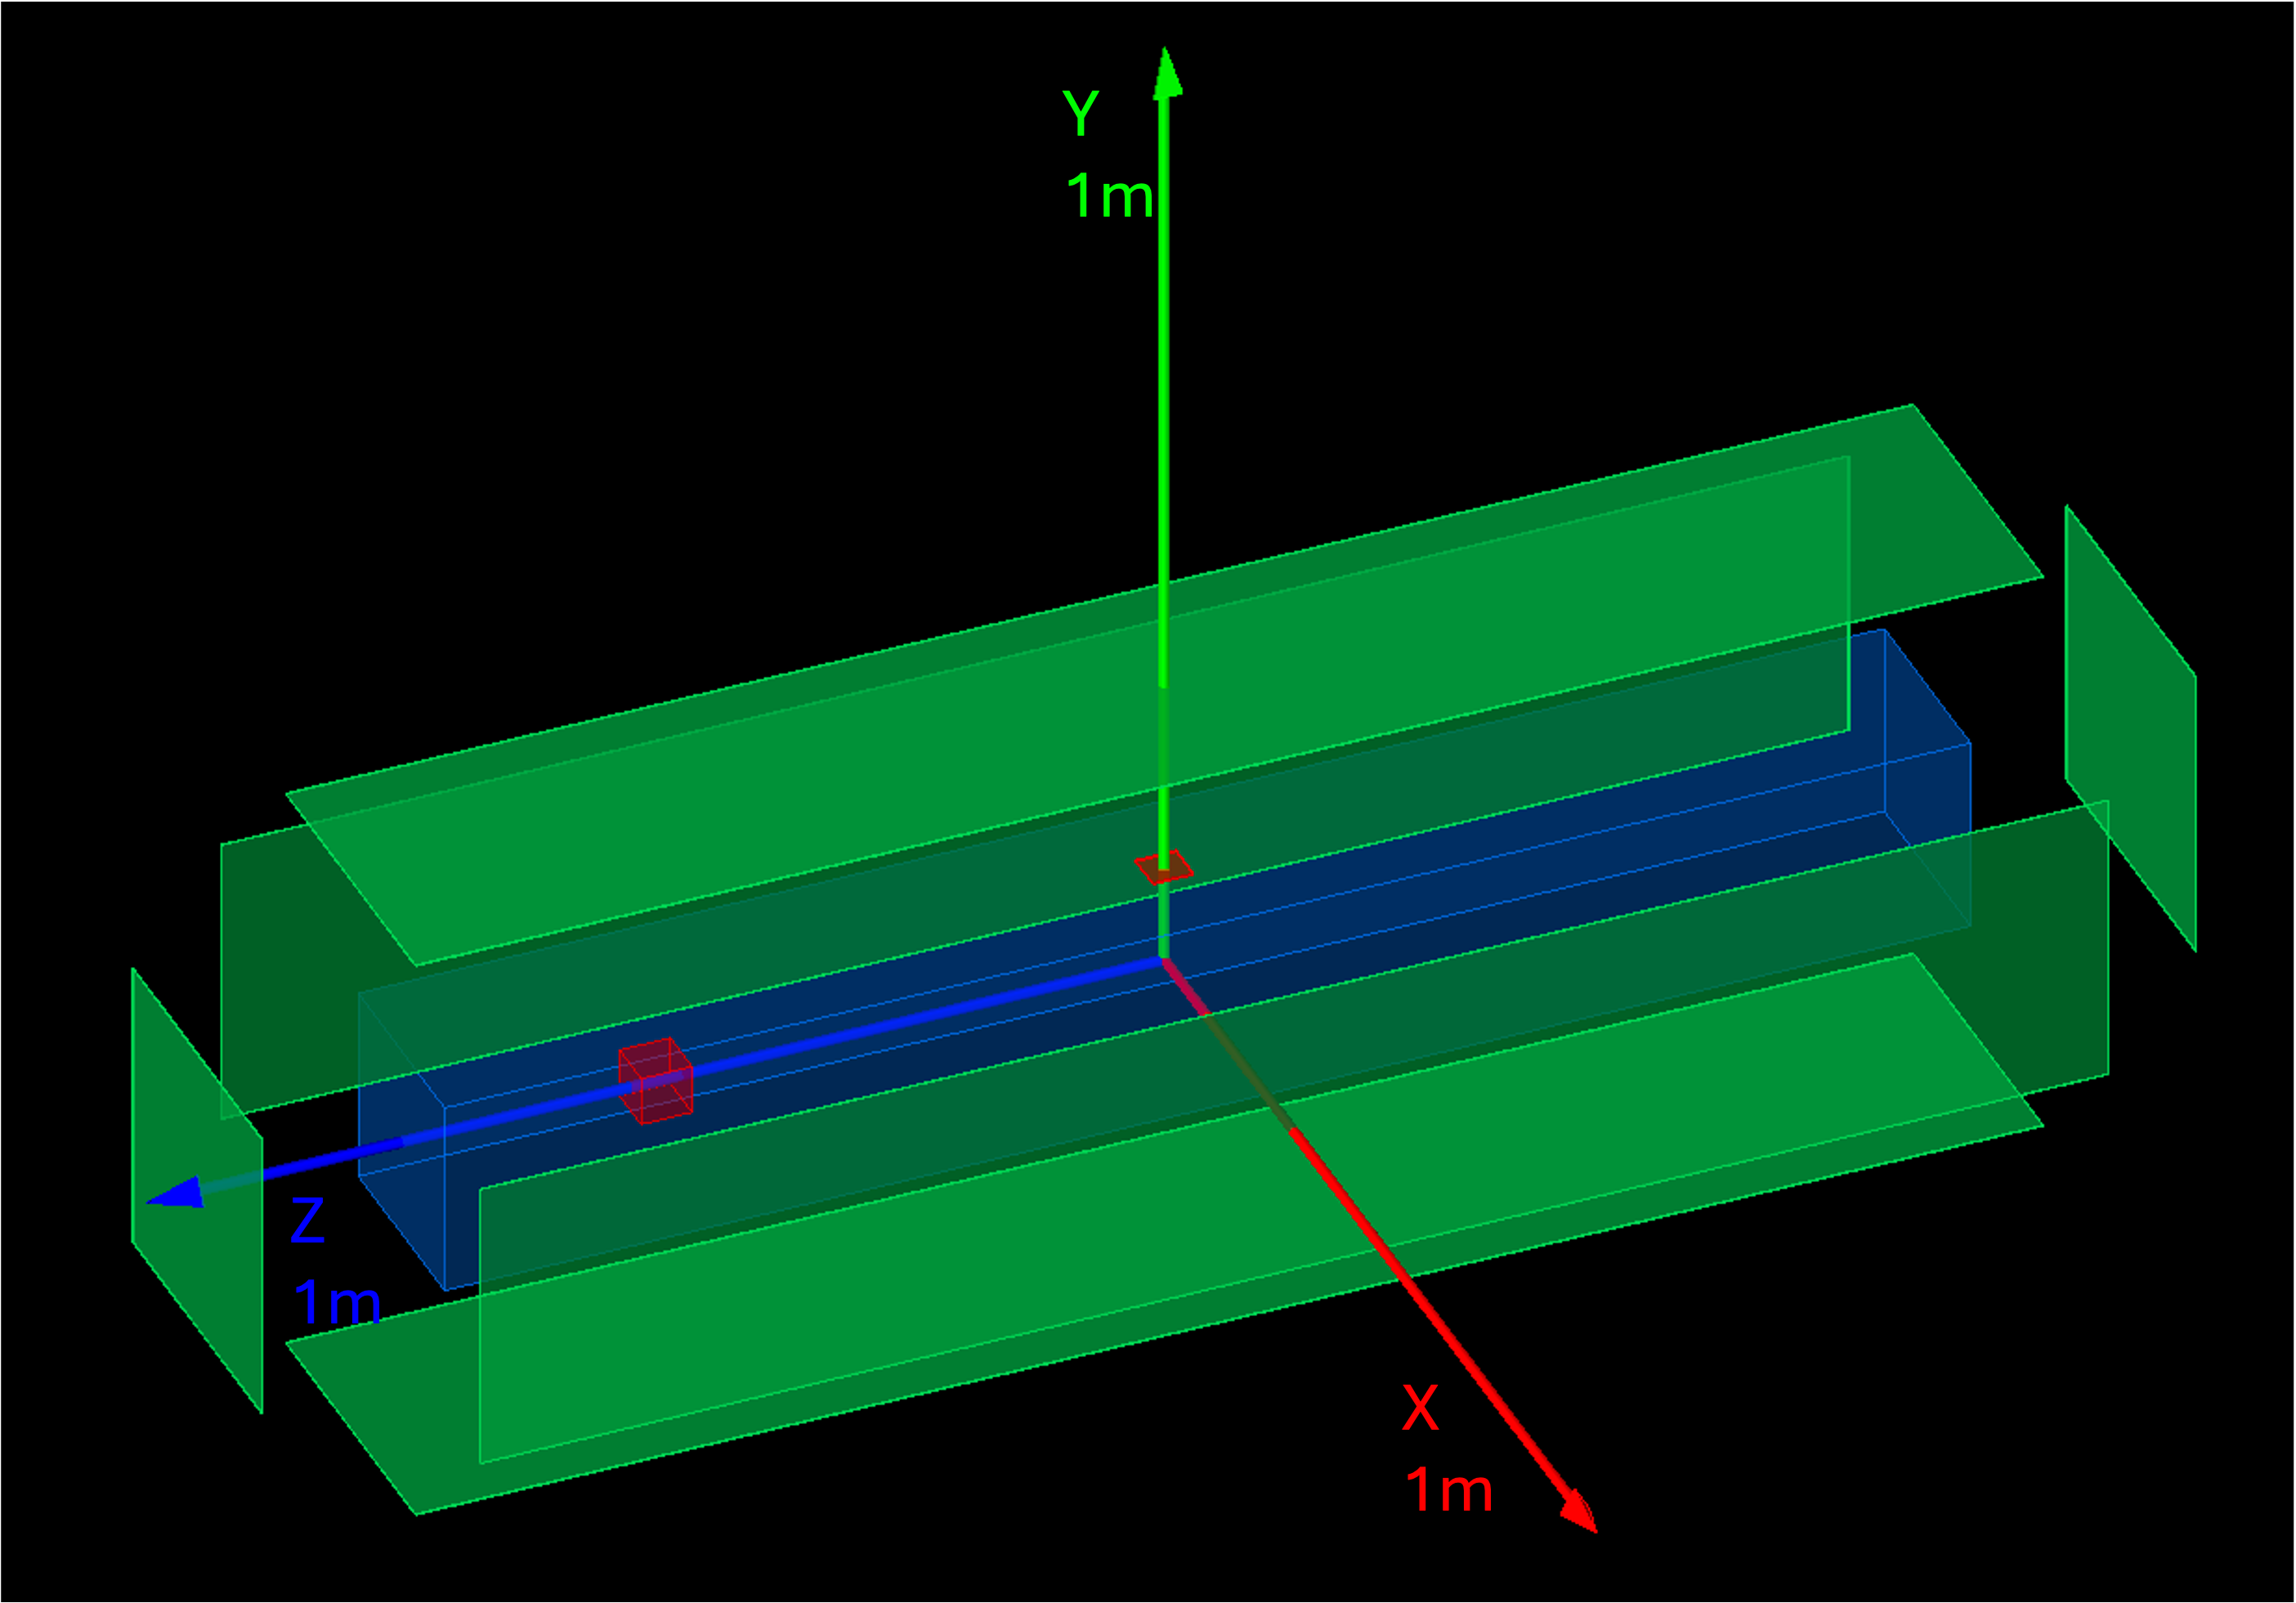
\includegraphics[width=0.5\linewidth]{geometry.png}
    \caption{Model geometry: water box (dark red), detector panels (green),
    and source regions (bright red) on the \(+y\) surface of the water box
    and displaced along the \(z\) axis inside the box.}
    \label{fig:geometry}
\end{figure}
The glue material is represented as cyanoacrylate with density
\(\SI{1.07}{\gram\per\cubic\centi\metre}\) and elemental composition
\(C_6H_7NO_2\).

\section{Physics and source model}

%The transport model includes low-energy electromagnetic interactions, radioactive decay-chain evolution, and step limiting.  The production-cut energy range is set to \(\SI{100}{eV}\) to \(\SI{1}{GeV}\), with a default cut value of \(\SI{1}{nm}\). 
Primaries are generated as stationary Rn-222 ions:
\[
  Z=86, \qquad A=222, \qquad E=\SI{0}{MeV}.
\]
Rn diffusion is represented by sampling a random direction and a
decay-time-dependent displacement scale
\[
  \Delta r \sim \left| \mathcal{N}\left(0, \sqrt{6Dt}\right) \right|,
\]
with \(D=\SI{1.12e-3}{\milli\metre\squared\per\second}\) for radon-222.
The glue slab side walls reflect the sampled displacement in \(x\) and
\(z\).  Motion out of the top of the glue is reflected, while motion below
the bottom glue boundary is logged as an Rn-222 glue-exit event.  The exit
log records event ID, track ID, estimated exit time, decay time, start
position, exit position, and final sampled position.

\section{Rn-222 decay simulations}

The repeated simulation campaign contains six source configurations, each with ten
independent repetitions and \(10{,}000\) simulated primary Rn-222 events per
repetition.  Each repetition uses a unique random seed.

\begin{table}[h]
\centering
\caption{Rn-222 source configurations in the repeated campaign.  The glue
source is a \(\SI{40}{mm} \times \SI{2}{mm} \times \SI{40}{mm}\) volume
centered at \((0,101,0)~\si{mm}\).  The diffuse water source is the full
water box.  The localised water source is a \(\SI{5}{cm}\)-side cube
centered at \((0,0,50)~\si{cm}\).}
\begin{tabular}{lll}
\toprule
Case & Glue fraction & Additional Rn-222 source \\
\midrule
baseline & 1.0 & none \\
$diff_{10}$ & 0.9 & 0.1 diffuse in water box \\
$diff_{50}$ & 0.5 & 0.5 diffuse in water box \\
$diff_{90}$ & 0.1 & 0.9 diffuse in water box \\
$loc_{40}$ & 0.6 & 0.4 localised in water cube \\
$loc_{60}$ & 0.4 & 0.6 localised in water cube \\
\bottomrule
\end{tabular}
\end{table}

\section{Analysis definitions}

The primary analysis records gamma entries and exits at the water volume,
glue volume, and detector plates.  The detector-response metrics in this
note use gamma entries into a photon detector plate.  Counts are therefore
detector-entry counts, not all emitted photons.  The analysis also reports
unique detected gamma-track counts within each event.  Profile and heatmap
comparisons use baseline-subtracted detector-entry histograms, with repeated
runs providing the uncertainty.

\section{Results}

\subsection{Total Detector Entries}

Table~\ref{tab:total-response} summarises the total detector entries per
\(10{,}000\) primary Rn-222 events.  The total response decreases from the
baseline to high water-distributed cases, but the change is small compared
with the much larger redistribution among detector panels shown below.

\begin{table}[h]
\centering
\caption{Mean detector-entry counts across ten repetitions.  Uncertainties
are standard deviations across repetitions.}
\label{tab:total-response}
\begin{tabular}{lccc}
\toprule
Case & Detector entries & Unique gamma tracks & Entries per primary event \\
\midrule
baseline & \(12500 \pm 82\) & \(12415 \pm 82\) & \(1.250 \pm 0.008\) \\
diff10 & \(12431 \pm 100\) & \(12349 \pm 97\) & \(1.243 \pm 0.010\) \\
diff50 & \(12300 \pm 130\) & \(12218 \pm 128\) & \(1.230 \pm 0.013\) \\
diff90 & \(12057 \pm 86\) & \(11981 \pm 87\) & \(1.206 \pm 0.009\) \\
loc40 & \(12174 \pm 79\) & \(12096 \pm 80\) & \(1.217 \pm 0.008\) \\
loc60 & \(12134 \pm 81\) & \(12058 \pm 80\) & \(1.213 \pm 0.008\) \\
\bottomrule
\end{tabular}
\end{table}

\subsection{Detector-Panel Redistribution}

Table~\ref{tab:panel-response} shows mean detector-entry counts by panel.
The baseline case is dominated by the positive-\(y\) plate because the glue
source lies immediately above the water box.  As more Rn-222 is assigned to
water, the positive-\(y\) excess is reduced and the negative-\(y\), \(x\),
and \(z\) panels receive larger fractions.  The localised water cases retain
the same qualitative behaviour but produce asymmetric \(z\)-panel responses
because the localised cube is placed at positive \(z\).  The corresponding
baseline-subtracted panel profiles and maps are shown in
Figs.~\ref{fig:y-profile}--\ref{fig:x-zscore}.

The residual profiles and heatmaps are constructed as
candidate-minus-baseline detector-entry histograms after applying the same
binning to both simulations.  In the two-dimensional maps, positive bins
indicate detector regions where the candidate configuration produces more
hits than the retained-source baseline, while negative bins indicate
regions depleted relative to baseline.  The z-score profiles divide the
same residuals by the repetition-derived uncertainty in each bin; they are
therefore a bin-wise signal-to-noise diagnostic rather than an independent
physical observable.

\begin{table}[h]
\centering
\caption{Mean detector-entry counts by detector panel across ten repetitions.}
\label{tab:panel-response}
\begin{tabular}{lrrrrrr}
\toprule
Case & NegX & PosX & NegY & PosY & NegZ & PosZ \\
\midrule
baseline & 2570 & 2594 & 1420 & 5882 & 18 & 16 \\
diff10 & 2622 & 2632 & 1550 & 5552 & 35 & 40 \\
diff50 & 2740 & 2743 & 2143 & 4412 & 133 & 130 \\
diff90 & 2851 & 2851 & 2736 & 3178 & 223 & 218 \\
loc40 & 2694 & 2683 & 1986 & 4663 & 11 & 136 \\
loc60 & 2741 & 2748 & 2315 & 4117 & 9 & 204 \\
\bottomrule
\end{tabular}
\end{table}

\begin{figure}[h]
\centering
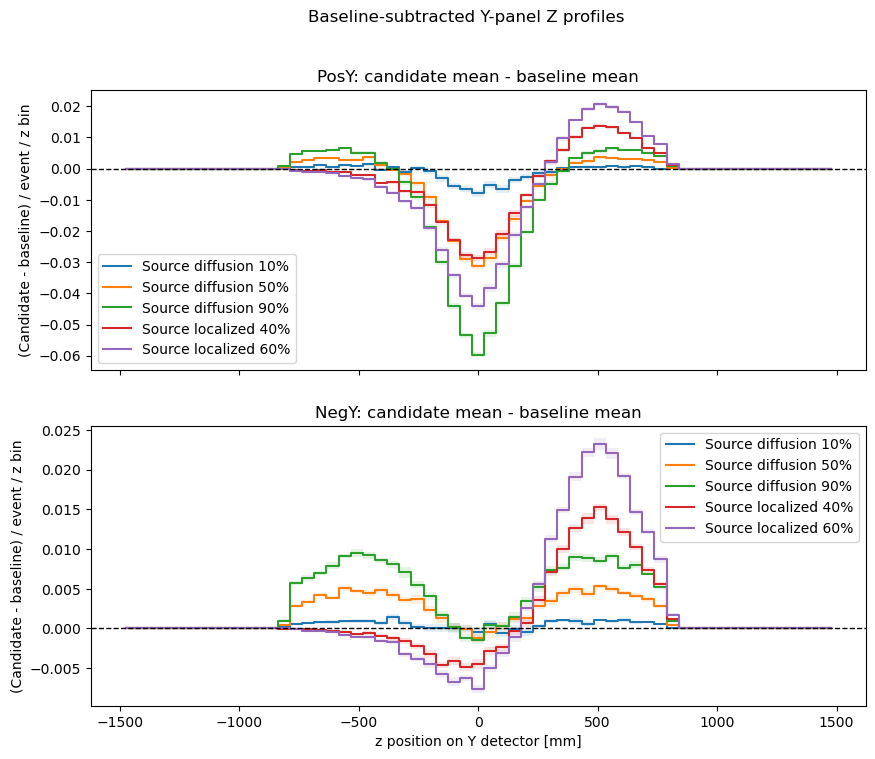
\includegraphics[width=\textwidth]{y_panel_baseline_subtracted_z_profiles.png}
\caption{Baseline-subtracted \(z\)-profiles for the positive-\(y\) and
negative-\(y\) detector panels.  Moving Rn-222 from the glue layer into
water changes the panel balance and produces a measurable residual structure
along the detector length.}
\label{fig:y-profile}
\end{figure}

\begin{figure}[h]
\centering
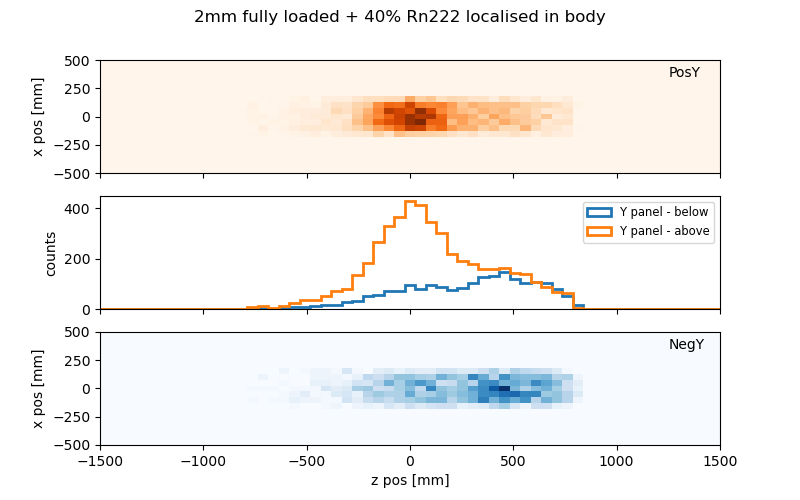
\includegraphics[width=\textwidth]{2mm_fully_40rn222loc_yprofile.png}
\caption{\(y\)-panel response profile for the localised water-source case
with 40\% of the activity in the localised water region.}
\label{fig:loc40-y-profile}
\end{figure}

\begin{figure}[h]
\centering
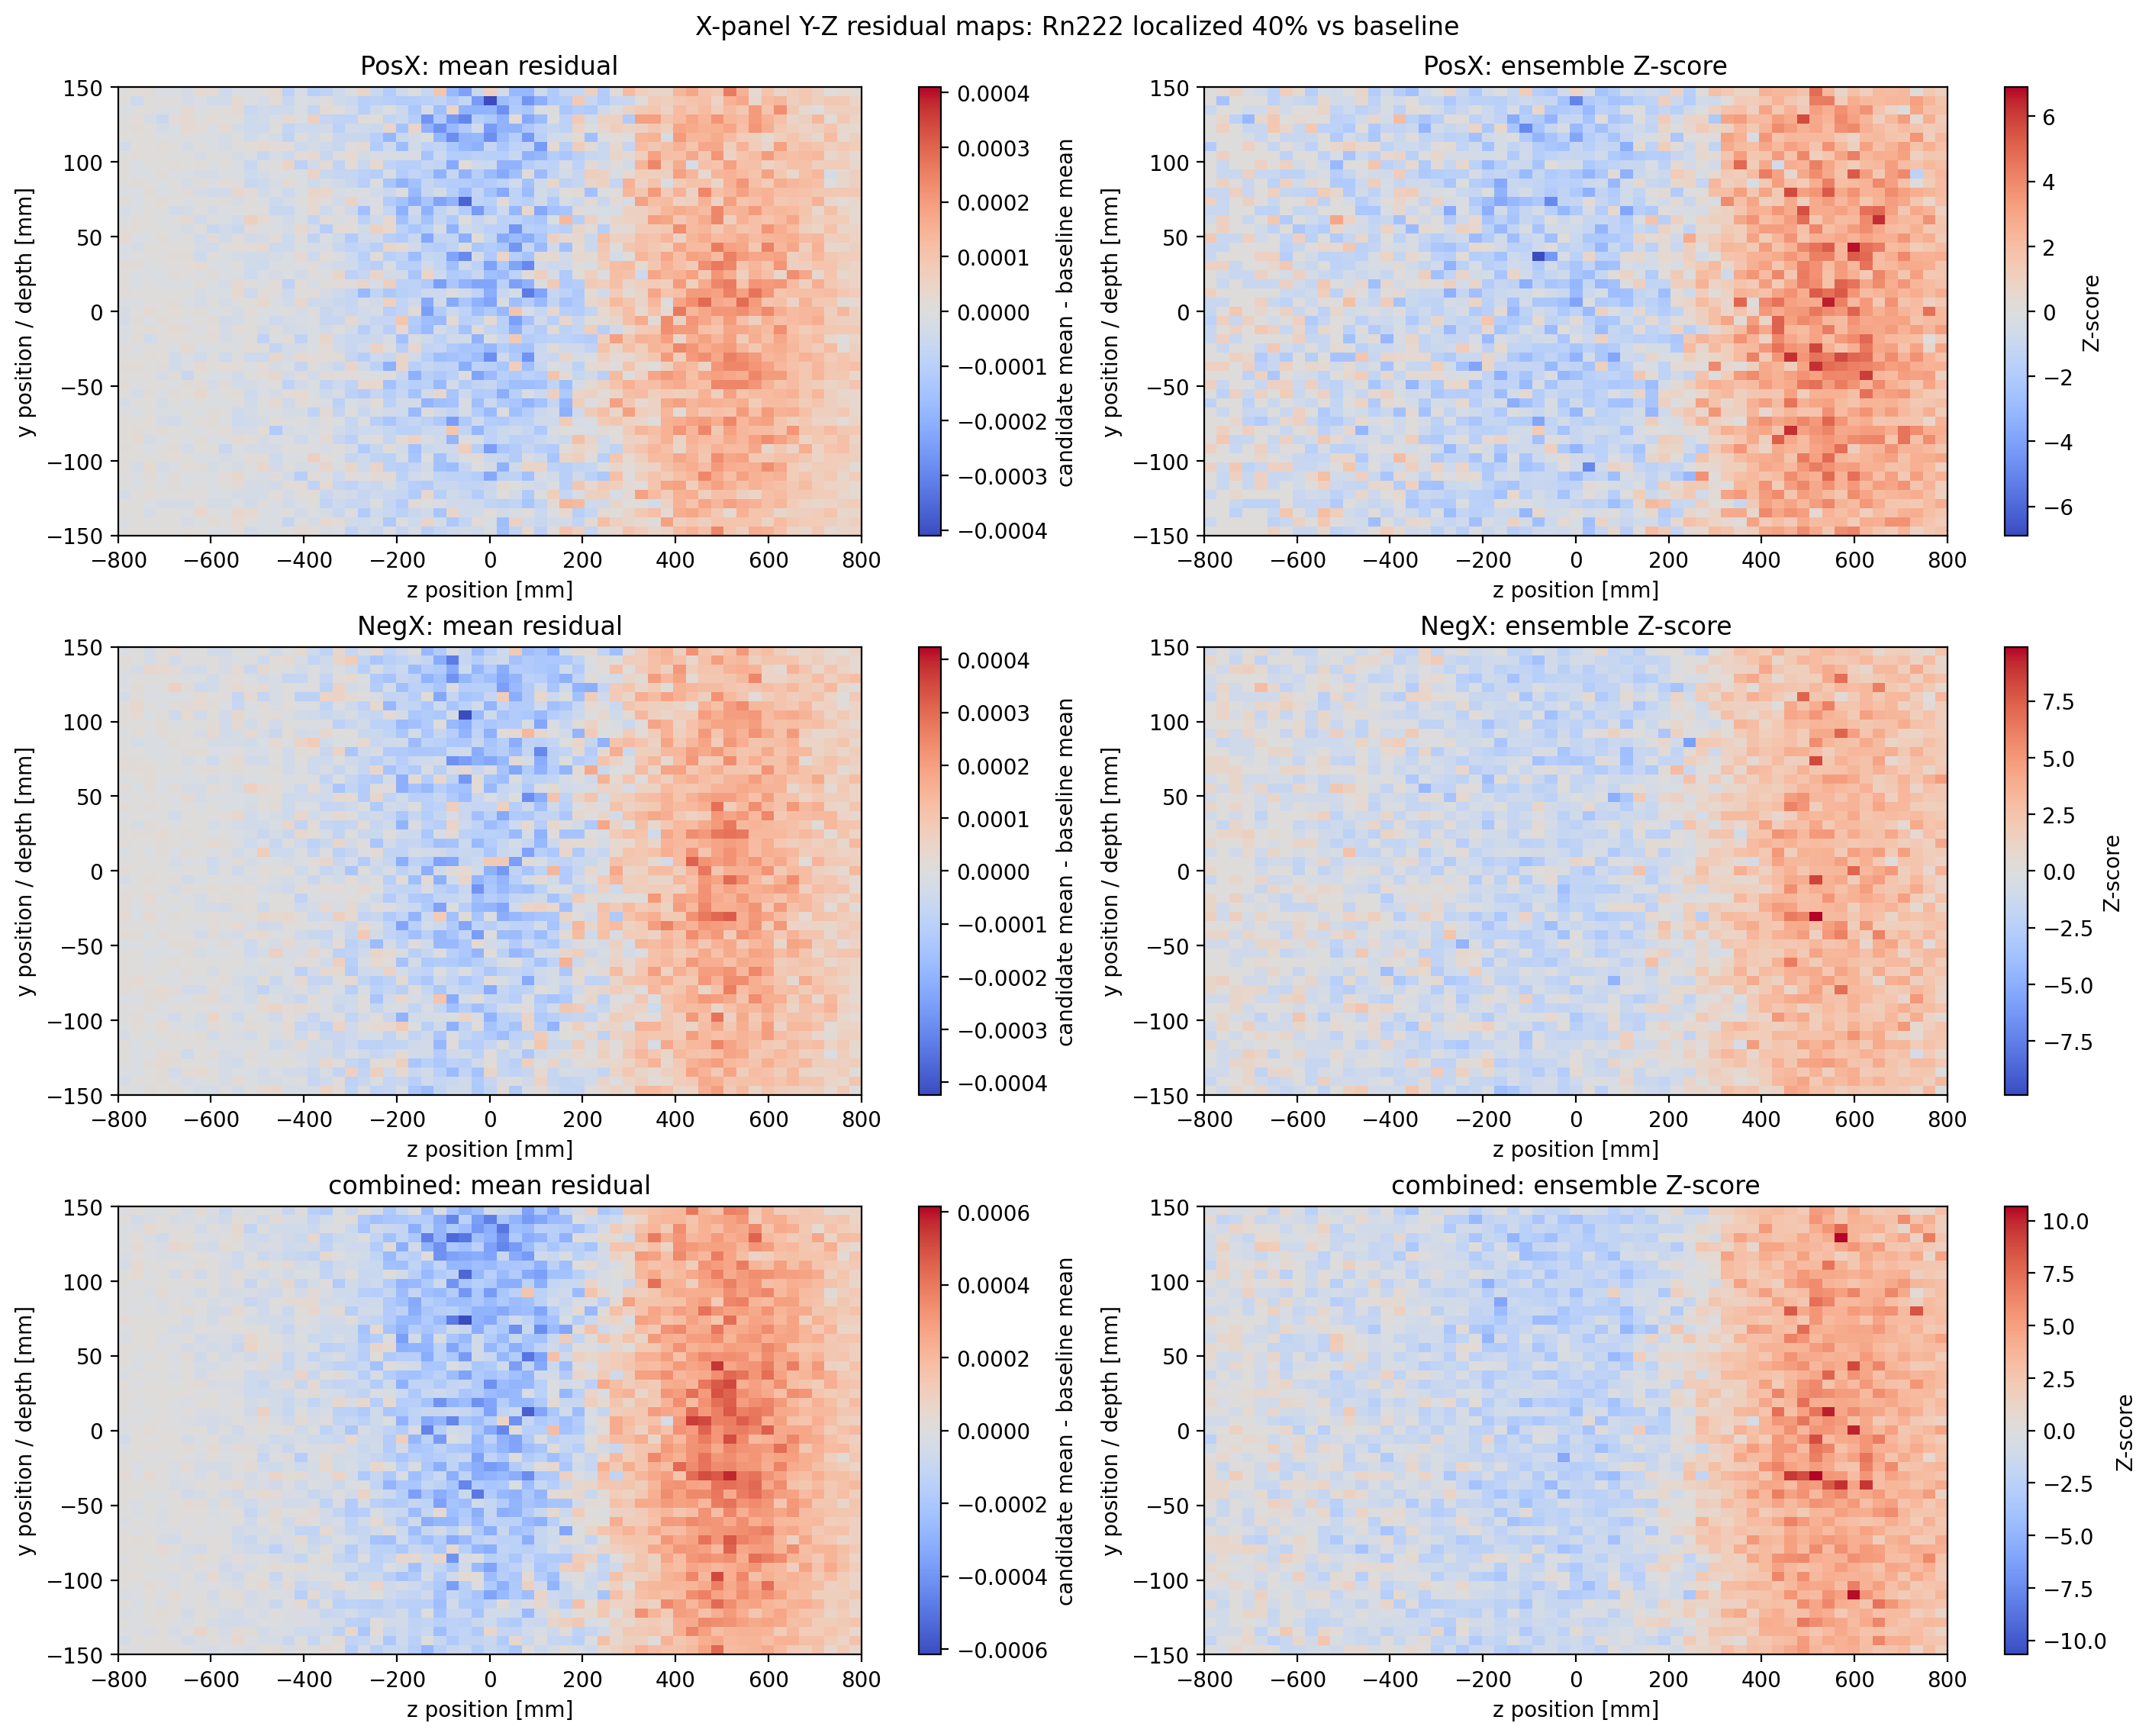
\includegraphics[width=\textwidth]{x_panel_yz_residual_maps_loc40.png}
\caption{\(x\)-panel \(y\)-\(z\) residual heatmaps for the localised
water-source case with 40\% of the activity in the localised water region.
The colour scale shows candidate-minus-baseline detector-entry counts in
each spatial bin.}
\label{fig:x-map}
\end{figure}

\begin{figure}[h]
\centering
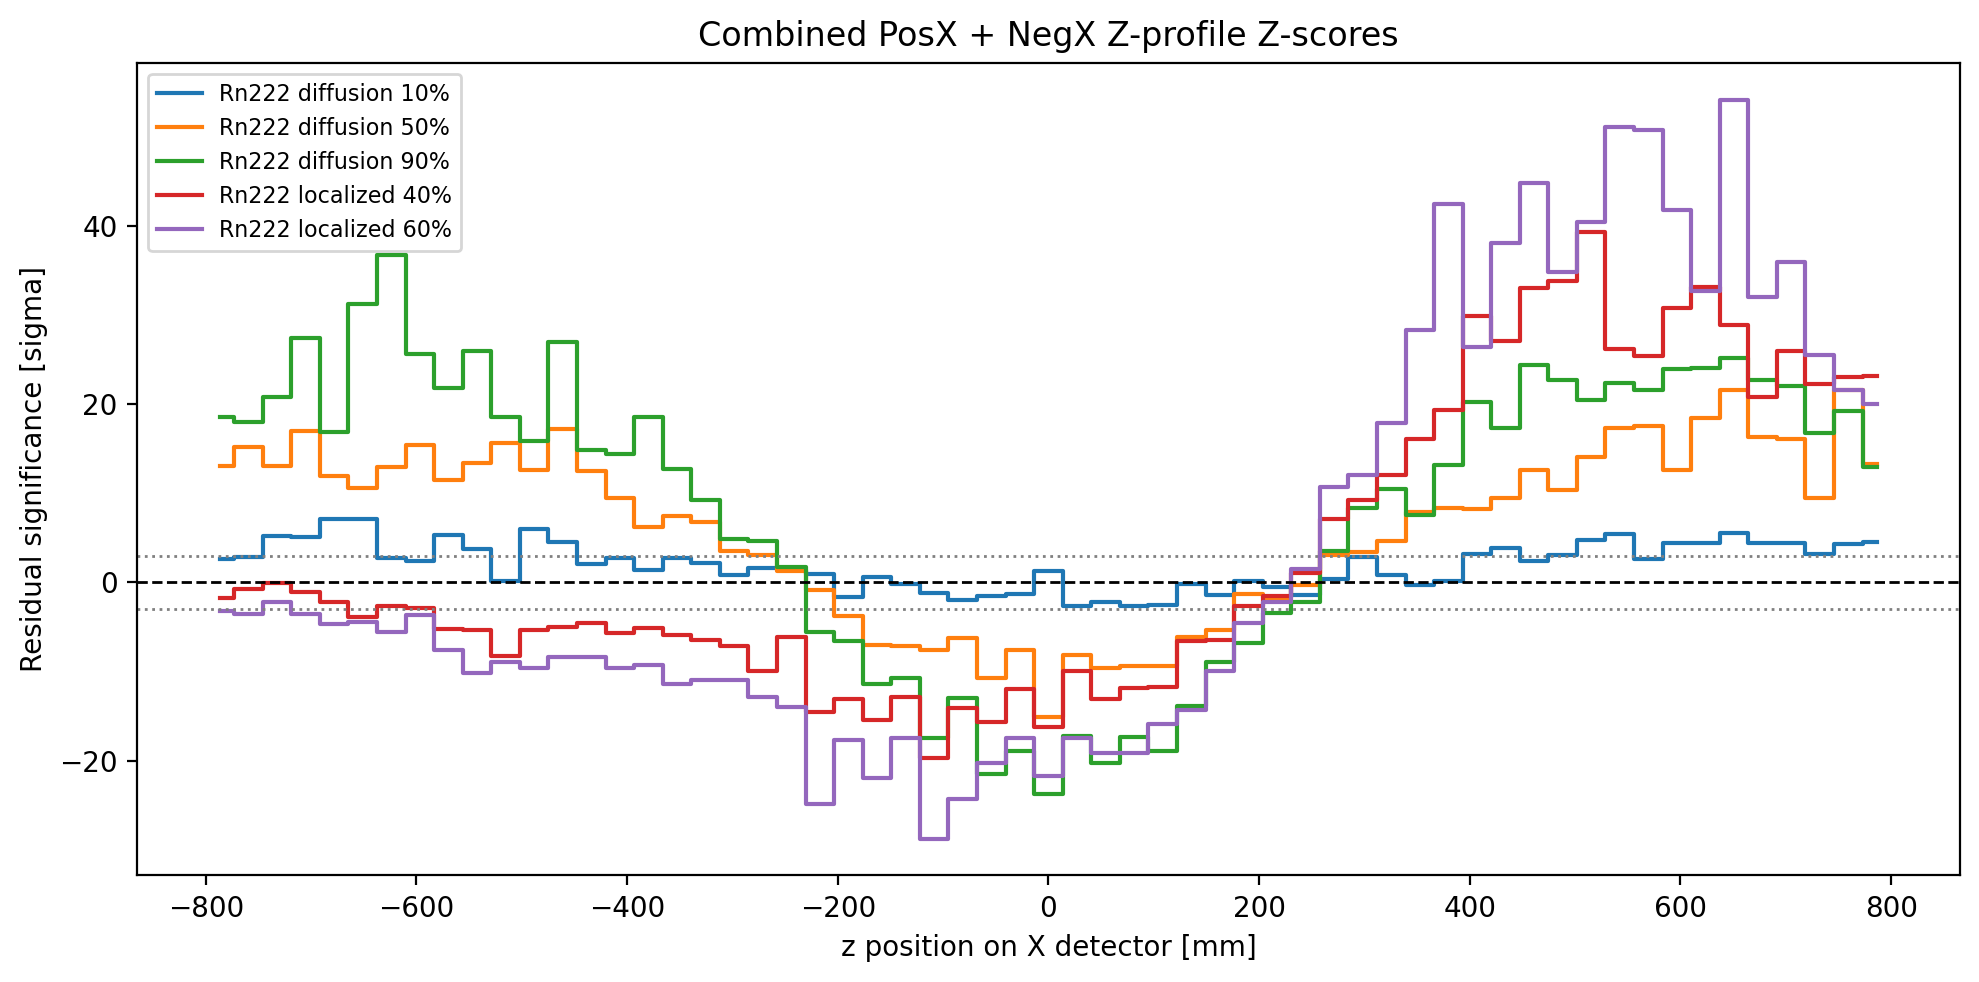
\includegraphics[width=\textwidth]{x_panel_z_profile_zscores.png}
\caption{\(x\)-panel \(z\)-profile residuals expressed as bin-wise z-scores.
Large positive or negative values mark detector-position bins where the
candidate-minus-baseline residual is large compared with the run-to-run
uncertainty.}
\label{fig:x-zscore}
\end{figure}

\subsection{Source-isotope attribution}

Across all Rn-222 configurations, detected photons are dominated by
late-chain gamma emitters.  In the baseline case, approximately
\(\SI{60.5}{\percent}\) of detector entries are attributed to Po-214,
\(\SI{37.1}{\percent}\) to Bi-214, and \(\SI{2.2}{\percent}\) to Bi-210 when
the full simulated time range is counted.  However, Bi-210 appears mainly at
late times in the decay chain and contributes little to the early
observation windows used for practical source-localisation analysis.  The
time spectrum in Fig.~\ref{fig:time-isotope} motivates the
\(t<10^6~\mathrm{s}\) analysis cut: it retains the Rn-222 progeny signal
from Po-214 and Bi-214 while excluding the much later Bi-210-dominated tail.
Pb-214 and other isotopes are present at low levels in the detector-entry
data.  Exploratory energy-spectrum checks by panel show the same late-chain
gamma-emitter population across the opposing detector faces, so the main
source-location information in this analysis comes from spatial hit
redistribution rather than from a change in the detected isotope mix.

\begin{figure}[h]
\centering
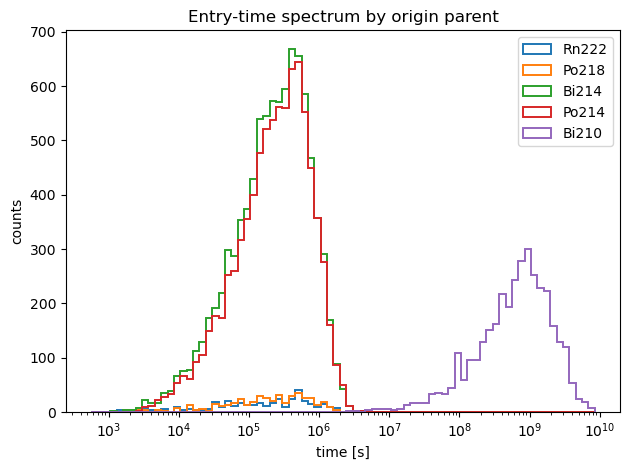
\includegraphics[width=0.82\textwidth]{Rn222-time-spectrum-by-isotope.png}
\caption{Detected-gamma time spectrum by source isotope.  The early response
is dominated by Po-214 and Bi-214, while Bi-210 appears primarily at much
later times; this motivates applying a \(t<10^6~\mathrm{s}\) cut when
focusing on treatment-relevant source-localisation windows.}
\label{fig:time-isotope}
\end{figure}

\subsection{Timing}

Cumulative time cuts show how many detector entries would be available as a
function of observation time.  For the baseline case, the mean cumulative
detector entries are \(29.5\) at 1 hour, \(106.3\) at 2 hours, \(977.8\) at 12 hours,
\(1933.3\) at 1 day, \(3639.8\) at 2 days, \(7217.8\) at 5 days, and \(10204.6\) at 10 days, per \(10{,}000\) simulated primaries.  The other source configurations follow similar time evolution with lower totals in
the high-water-fraction cases.  The development of the
baseline-subtracted spatial profile with cumulative observation window is
shown in Fig.~\ref{fig:time-profiles}.

\begin{figure}[h]
\centering
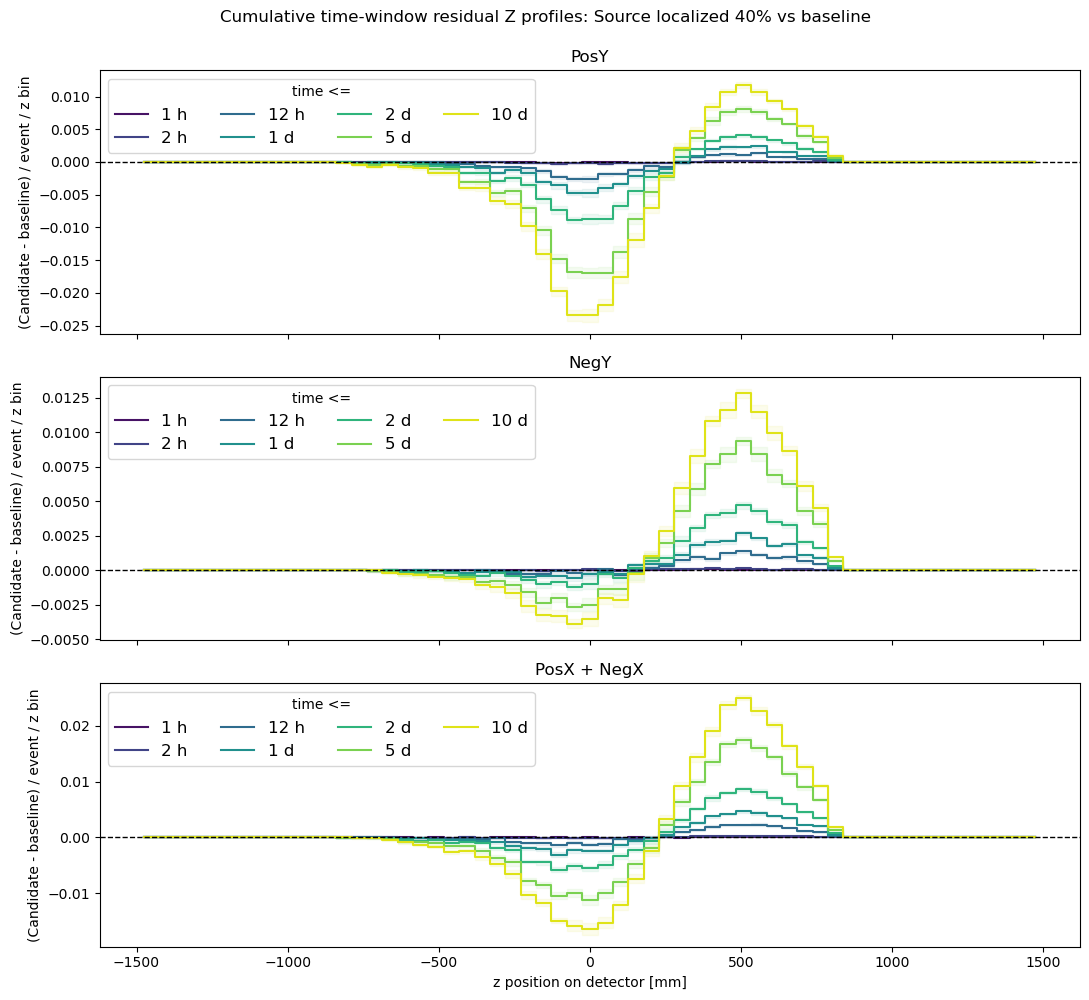
\includegraphics[width=\textwidth]{time_window_residual_z_profiles_loc40.png}
\caption{Cumulative time-window residual \(z\)-profiles for the localised
water-source case with 40\% of the activity in the localised water region.
The panels show how the baseline-subtracted profile develops as the
observation window increases.}
\label{fig:time-profiles}
\end{figure}

\subsection{Rn-222 glue exit}

The dedicated Rn-222 exit log records how often sampled Rn-222 motion
crosses the bottom of the glue slab before decay.  In the all-glue baseline
case, \(4593 \pm 50\) Rn-222 tracks per \(10{,}000\) primaries exit the glue
in the logged downward direction.  The mean repetition-level median exit
time is \(4.81 \pm 0.13\) hours, while the mean 90th-percentile exit time is
\(32.64 \pm 1.27\) hours.  As expected, the number of glue-exit records
scales down with the simulated fraction of Rn-222 initially assigned to the
glue layer: \(4094 \pm 41\) for diff10, \(2278 \pm 46\) for diff50, and
\(456 \pm 18\) for diff90.

\section{Comments}

The current simulation and analysis support three conclusions.
First, the detector system is sensitive to source placement through panel
balance: total counts alone are a weak discriminator, but the relative
response of \(+y\), \(-y\), \(x\), and \(z\) plates changes systematically.
Second, the dominant detected gamma population comes from Po-214 and Bi-214,
so isotope attribution mainly confirms the expected Rn-222 decay chain
rather than separating the spatial hypotheses.  Third, the logged diffusion
model predicts substantial Rn-222 movement from the glue into water on
hour-scale times, which is consistent with the need for cumulative
time-window analysis and activity-normalised projections.

\section{Limitations and next steps}

The current tabulated analysis treats detector entries as ideal photon hits.
It does not yet include detector efficiency, energy resolution, coincidence
logic, electronic thresholds, or measured background.  The back-projection
analysis estimates source-track proxies from detector-entry position and
momentum, but a single gamma constrains a line rather than a unique source
point.  A stronger reconstruction study should combine detector response
maps with a likelihood model over source distributions and should include
the detector-response model needed for comparison with data.  A further next
step is to replace the present normalisation by total simulated event count
with an activity-based normalisation, so that profiles and time windows can
be interpreted as expected detector hits for a specified source activity.

\end{document}
